\documentclass[a4paper,11pt]{ltjsarticle}
\usepackage{graphicx}
\usepackage{luatexja-fontspec}
\usepackage{caption}
\usepackage{amsmath,amssymb,bm,braket}
\usepackage[english]{babel}
\usepackage{multicol}
\usepackage{titlesec}
%\usepackage{gnuplot-lua-tikz}
\usepackage[top=20truemm,bottom=20truemm,left=20truemm,right=20truemm]{geometry}
\usepackage{array}
\usepackage{upgreek}
\usepackage{fancyhdr}
\renewcommand{\refname}{}
\usepackage{listings,jvlisting}
\usepackage{tikz}
\usepackage[thmmarks,amsmath]{ntheorem}
\usepackage[version=3]{mhchem}
\usetikzlibrary{external}
\tikzexternalize
\lstset{
  basicstyle={\ttfamily},
  identifierstyle={\small},
  commentstyle={\smallitshape},
  keywordstyle={\small\bfseries},
  ndkeywordstyle={\small},
  stringstyle={\small\ttfamily},
  frame={tb},
  breaklines=true,
  columns=[l]{fullflexible},
  numbers=left,
  xrightmargin=0pt,
  xleftmargin=3pt,
  numberstyle={\scriptsize},
  stepnumber=1,
  numbersep=1pt,
  lineskip=-0.5ex
}
\captionsetup[figure]{format=plain, labelformat=simple, labelsep=quad,labelfont=bf,name={Fig.}}
\captionsetup[table]{format=plain, labelformat=simple, labelsep=quad,labelfont=bf}
\parindent = 0pt
%[BoldFont=HGSMinchoE]{MSMincho}[BoldFont=HiraMinProN-W6]{HiraMinPro-W3}
\titleformat{\section}{\normalfont\fontsize{9}{10}\bfseries\fontspec{Times New Roman}}{\thesection.}{1em}{}
\usepackage[backend=biber,sorting=none,style=numeric,maxnames=99,minnames=1]{biblatex}
\addbibresource{utility/REFERENCES.bib}
\defbibheading{bibliography}[\refname]{%
  \section*{REFERENCES}%
  \vspace{-7pt}  % ここで空白を調整。お好みの値に変更してください。
}
\newfontfamily\subsectionfont{Times New Roman} % サブセクション用フォント
\titleformat{\subsection}
  {\normalfont\large\bfseries} % サブセクションのフォントを指定
  {\thesubsection}{1em}{}
\renewbibmacro{in:}{}
\renewbibmacro*{journal+issuetitle}{%
  \addcomma\space% カンマとスペースを追加
  \usebibmacro{journal}%
  \setunit*{\addspace}%
  \usebibmacro{volume+number+eid}%
  \setunit{\addspace}%
  \printfield{note}%
  \newunit
}
\renewbibmacro*{volume+number+eid}{
  \printfield{volume}%
  \setunit*{\addnbspace}%
  \printfield{number}%
  \setunit{\addcomma\space}%
  \printfield{eid}
}
\DeclareFieldFormat[article]{volume}{\textbf{#1}}
\DeclareFieldFormat[article]{pages}{#1}
\DeclareFieldFormat{journaltitle}{#1}
\usepackage{hyperref}
\renewenvironment{abstract}{\par\noindent}{\par}
%\pagenumbering{gobble}
\usepackage{docmute}
\usepackage{setspace}
\usepackage{titlesec} % 見出しのカスタマイズ用

% セクションのフォーマットをカスタマイズ
\titleformat{\section}
  {} % フォントサイズとスタイル
  {\Large\bfseries\thesection\ \ }               % 番号の前の内容(空白)
  {0em}            % 番号とタイトルの間の間隔
  {\Large\bfseries}


\theoremstyle{plain}
\theoremheaderfont{\normalfont\bfseries}
\theorembodyfont{\itshape}   % 本文を斜体に
\theoremseparator{.}         % タイトルと本文の区切りを「.」に設定
\newtheorem{definition}{Definition}
\begin{document}
\section{Looped Pipeline Architecture}\label{looped_pipeline}{
    \ \ \ Many quantum computing platforms are based on a two-dimensional physical layout. We focus on "looped pipelines," \cite{cai2023} which offer the advantages of a three-dimensional lattice while being restricted to two-dimensional space. This architecture leverages qubit shuttling, where qubits are moved around on the chip, enabling long-range interactions between qubits that are far apart. 

    \subsection{Classical Linear Pipeline}{

        \begin{figure}[h]
            \centering
            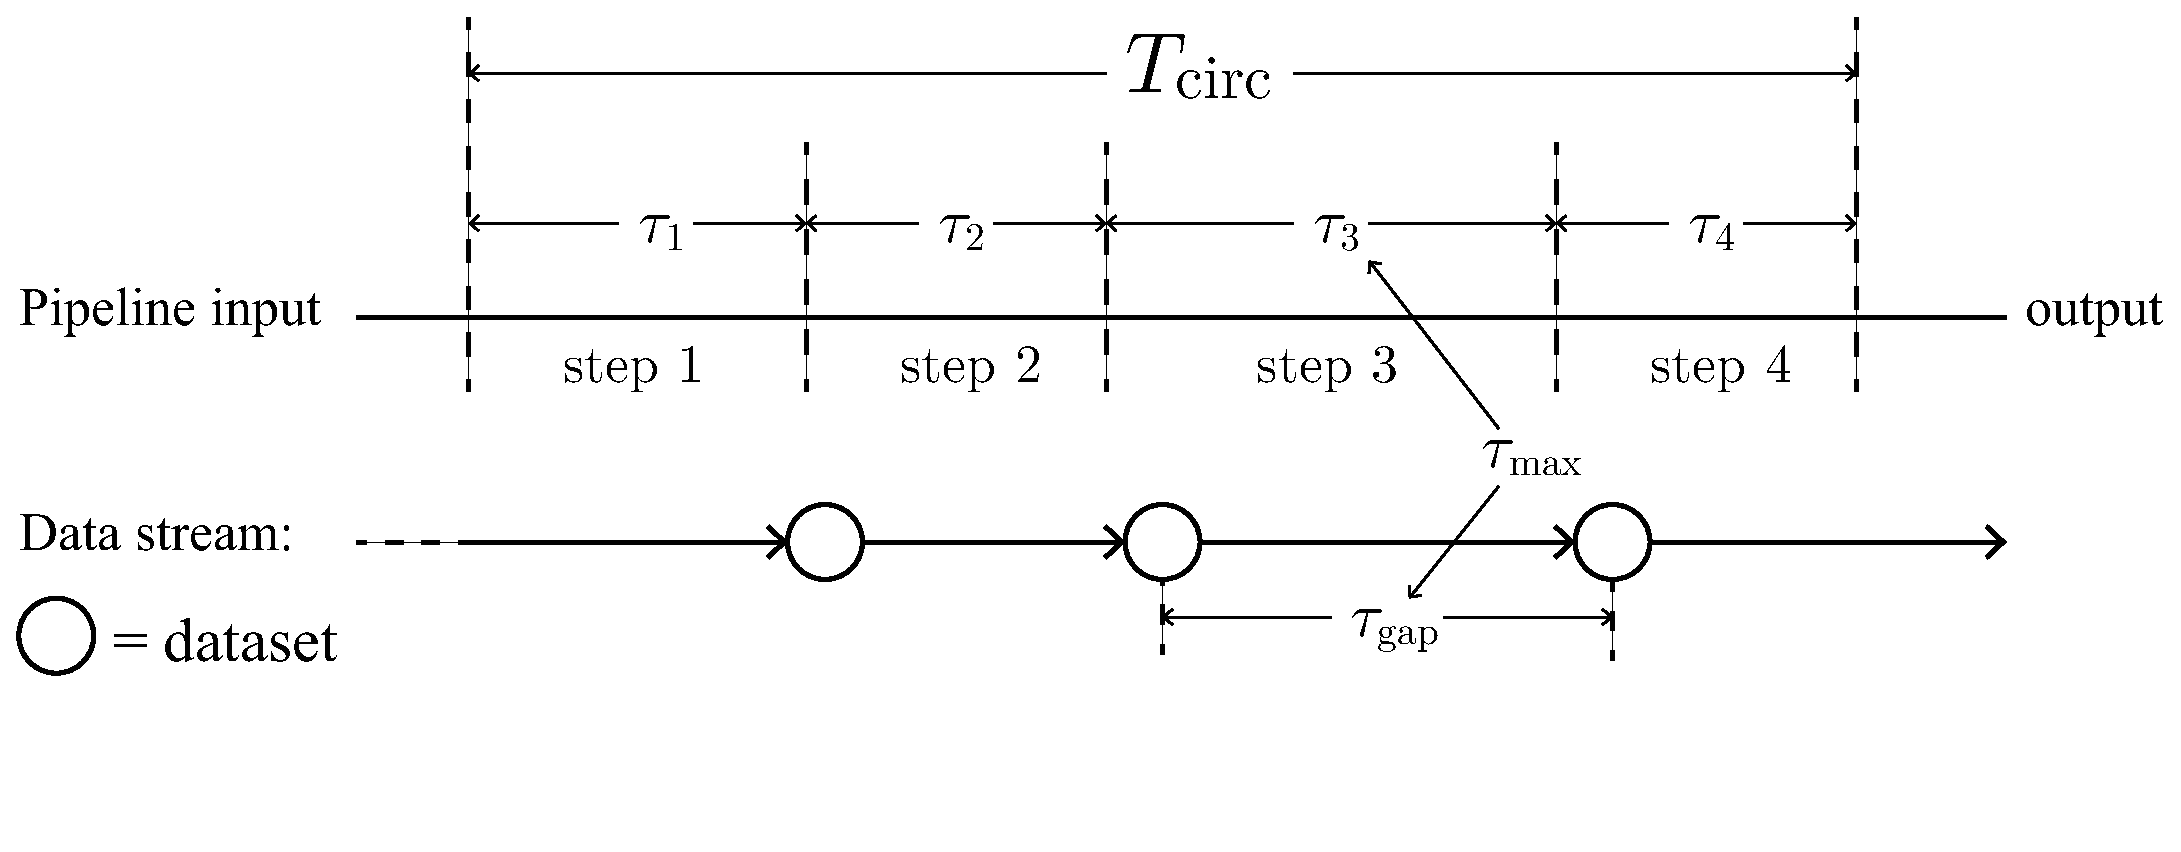
\includegraphics[scale=0.40]{figure/classical_pipeline.eps}
            \vspace{-20pt}\caption{An example of a classical data pipeline consists of four steps. Here, there is a steady flow of datasets with a time gap of $\tau_{\max}$ between consecutive datasets.}
            \label{classical_pipeline}
            \vspace{-10pt}
        \end{figure}

        \ \ \ Let us fist introduce "data-processing pipeline," we divide data-processing circuit into multple steps with each step able to operate only one dataset at a time shown in Fig.~\ref{classical_pipeline}. Now intead of inputting second dataset after the processing the first dataset on whole circuit, we input it as soon as finishing the process of the first dataset on step 1, similarly all subseaquent datasets and subseaquent steps. In this way, all data-processing steps can be working on different datasets in parallel, increasing the throughput of the system. this is a concept of pipelining. 
        \ \ \ The processing time of the $m$th step is denoted as $\tau_m$, and suppose there exist $M$ steps in the circuit. Then, the total time $T_{\text{circ}}$ taken for the entire circuit to process one dataset is given by:
        \begin{align}
            T_\text{circ}=\sum_{m=1}^M\tau_m.
        \end{align}
        This is the time required for every dataset without pipelining, and it is also the time required to process the first dataset in pipelining. For the second dataset in pipelining, the additional time required for processing is given by:
        \begin{align}
            \tau_\text{max}=\max_i{\tau_i}.
        \end{align}
        which is called "rate-limiting step." From the second dataset onward, the time required for processing each dataset equals the maximum of $\tau_i$. Hence, the total time for processing the $k$th datasets are given by:
        \begin{align}\label{pipeline_processing_time}
            T_\text{pipe}=T_\text{circ}+(k-1)\tau_\text{max}.
        \end{align}
        We call this the "steady-flow" pipelining scheme, as the data stream can flow through the entire pipeline without requiring modifications to the time gap between adjacent datasets or being put on hold at any point along the pipeline. Deviating from the steadyflow scheme, we often need to tempolary put the dataset on hold in the pipeline. For this, we need to implement "baffer" where multiple datasets can be on hold. 
    }
    \subsection{Looped Qubit Pipeline}{
        \begin{figure}[h]
            \centering
            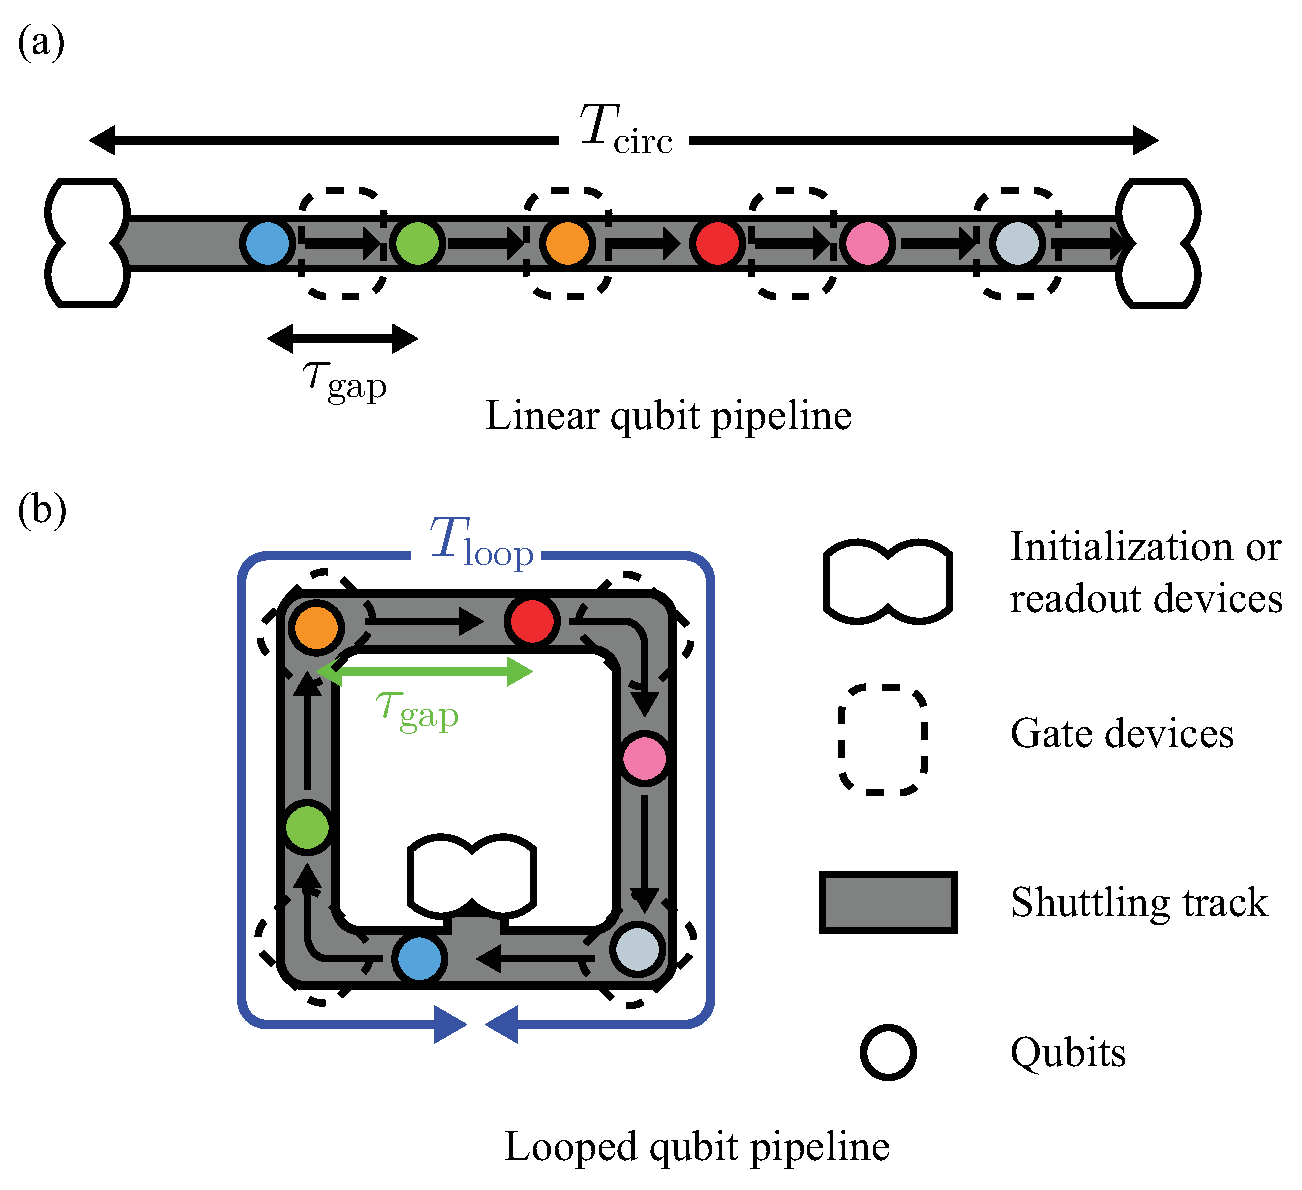
\includegraphics[scale=0.45]{figure/shuttling_track.eps}
            \vspace{0pt}\caption{Pipelines for applying single-qubit circuits to a stream of qubits.}
            \label{shuttling_truck}
        \end{figure}

        \ \ \ Similar to the classical pipeline, we can define the linear qubit pipeline, as shown in Fig.~\ref{shuttling_truck}(a). The qubits are processed at each step, which consists of shuttling, gate operations, initialization, or measurement. We can apply the steady-flow scheme to this pipeline, so the time required to process $k$ qubits is given by Eq.~\ref{pipeline_processing_time}. Note that, in practice, the rate-limiting step is often not the shuttling step, as the shuttling operation is relatively faster compared to other operations. Without loss of generality, we assume that the shuttling operation can hold the qubits without pushing them forward, allowing it to act as a buffering region for the pipelining when needed.\\
        \ \ \ Beyond the linear qubit pipeline, we can define the looped qubit pipeline, as shown in Fig.~\ref{shuttling_truck}. Unlike the linear qubit pipeline, where the circuits that can be performed on the qubits are restricted by the number of devices on the pipeline, the looped pipeline allows the qubits to circulate around the loop and reuse the gate devices. This enables the effective execution of circuits with any depth on the qubits. Focusing on the first qubit in the qubit stream, the time for wrapping around the loop is called the "cycling period," denoted as $T_\text{loop}$. Let us assume that all the additional qubits in the pipeline follow behind with a constant time gap $\tau_\text{gap}$ between consecutive qubits. To avoid a qubit collision, where the first qubit collides with the last qubit after wrapping around the loop, we need to ensure that the cycling period $T_\text{loop}$ is larger than the time gap between the first qubit and the last qubit, which is $(k-1)\tau_\text{gap}$, where $k$ is the number of qubits:
        \begin{align}
            T_\text{loop}\ge (k-1)\tau_\text{gap}.
        \end{align}
        The cycling period $T_\text{loop}$ may vary from one round to another because, for example, we might apply four gates in one round but only three gates in the next round, or certain rounds may not involve measurement or initialization. Let us denote the "minimum cycling period" throughout the entire pipeline process as $T_\text{loop}^\text{min}$. To avoid collisions, the following condition must hold:

        \begin{align}
            T_\text{loop}^\text{min}\ge (k-1)\tau_\text{gap},\\
            k\leq T_\text{loop}^\text{min}/\tau_\text{gap} + 1 = K_\text{loop}
        \end{align}

        where $K_\text{loop}$ represents the maximum number of qubits that can fit in the pipeline. In the steday-flow scheme, we have $\tau_\text{gap} = \tau_\text{max}$. thus, the maximum number of qubits that can fit in the loop in this case is:
        \begin{align}
            K_\text{loop} = T_\text{loop}^\text{min}/\tau_\text{max} + 1.
        \end{align}

        We can increase the number of qubits in the pipeline by reducing $\tau_\text{max}$. When the rate-limiting step is measurement or initialization, we can reduce their effective processing time by adding more initialization or measurement devices, as shown in Fig.~\ref{more_devices}, and operating them in parallel. If there are $m$ times more initialization or measurement devices in the pipeline, the rate-limiting time $\tau_\text{max}$, which represents the effective measurement or initialization time in parallel, will be reduced by a factor of $m$, provided we are operating on more than $m$ qubits: $\tau_\text{max} = \tau_\text{init/meas}/m$. This makes it possible to reduce $\tau_\text{max}$ to the extent that measurement or initialization is no longer the rate-limiting step.

        \begin{figure}[h]
            \centering
            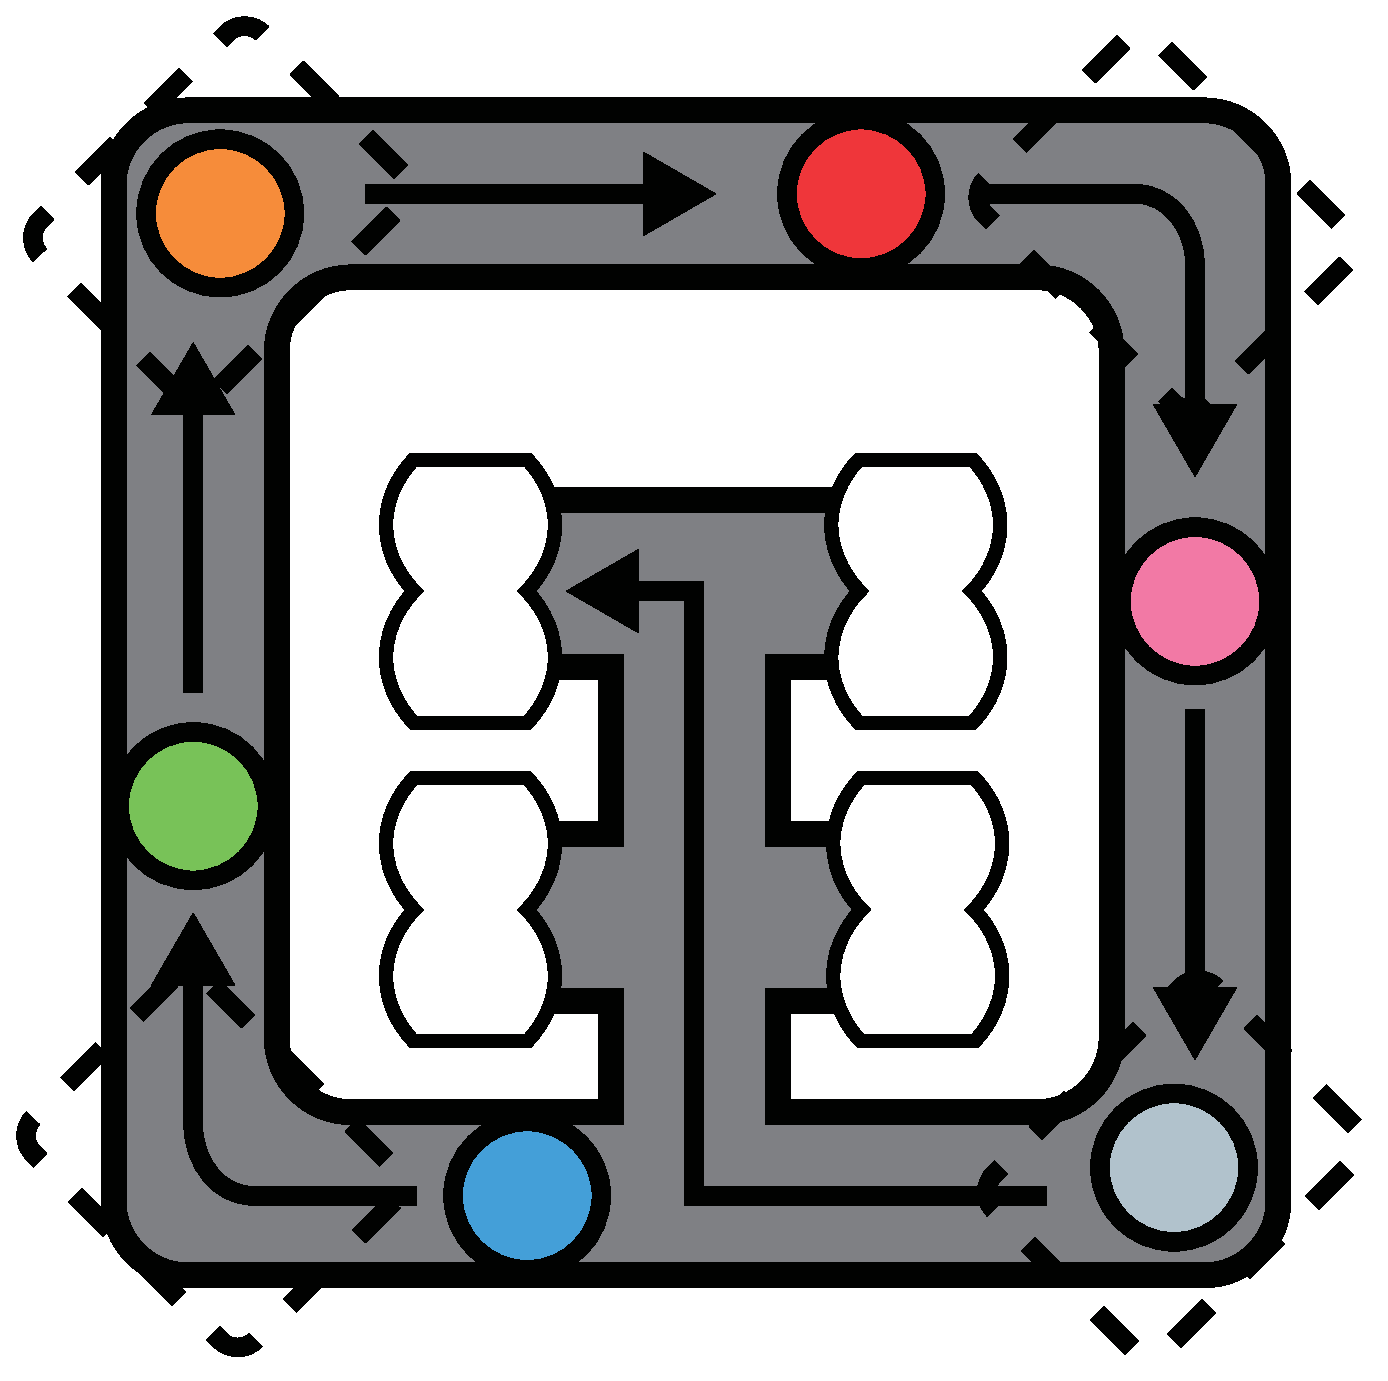
\includegraphics[scale=0.15]{figure/more_devices.eps}
            \vspace{0pt}\caption{Example of a looped qubit pipeline with multiple
            initialization or measurement devices.}
            \label{more_devices}
        \end{figure}
    }
}
\end{document}